%==============================================================================
%  MATH 231 -- Linear Algebra I (Queens College, Fall 2026)
%  MATRIX UNIT, PART 2 -- Column Space, Row Space, Rank, and the 2x2
%  Determinant
%
%  Section numbering runs CONTINUOUSLY across the parts of the matrix unit
%  (it restarted at 1 in Part 1, which opened the unit):
%
%      Part 1   MATH231_matrices_1_linear_systems_and_matrix_notation  Sec. 1-9
%      Part 2   MATH231_matrices_2_column_space_rank_and_the_determinant  10-14
%      Part 3   MATH231_matrices_3_matrices_that_move_the_plane           15-21
%      Part 4   MATH231_matrices_4_area_and_rotation                      22-25
%      Part 5   MATH231_matrices_5_projections_and_direct_sums            26-29
%      Part 6   MATH231_matrices_6_null_space_and_rank_nullity            30-34
%      Part 7   MATH231_matrices_7_the_determinant                        35-39
%      Part 8   MATH231_matrices_8_gaussian_elimination                   40-45
%      Part 9   MATH231_matrices_9_least_squares                          46-49
%      Part 10  MATH231_matrices_10_the_inverse_and_the_pseudoinverse     50-54
%      Part 11  MATH231_matrices_11_gram_schmidt_and_qr                   55-58
%
%  Hence \setcounter{section}{9}: this part opens at Section 10.
%
%  STATUS: complete.  Sections 10-14.  Written from the plan in
%  plan/MATH231_remaining_units_plan.tex (2026-10-25); the decisions below are
%  numbered as there.
%
%  AUDIENCE: distributed to students.  Keep it free of instructor-facing
%  apparatus -- time budgets, pacing notes, teaching cues.
%
%  DECISIONS CARRIED FROM THE PLAN.
%
%   D1. Part 1's closing Looking-ahead says Gaussian elimination is next.  In
%       the instructor's order it is Part 8.  Part 1 is left untouched; the
%       opening of this part explains the detour instead (when a solution
%       exists comes before how to find it).
%
%   D4. Row rank = column rank is CHECKED here for 2x2 only (Sec. 12.4: the
%       number ad - bc is the same read along rows or columns) and PROVED in
%       general in Sec. 33.3, as a corollary of rank(A'A) = rank(A).
%
%   D11. Sec. 13 keeps to matrices acting on R^n: the function x -> Ax, its
%       linearity, and "column j is where e_j goes".  General linear maps, and
%       the derivation of the product rule from composition, are left to the
%       end of the course; Sec. 13.3 says so in one remark.
%
%  NOTATION (plan N1, N2).  col[A], row[A] as used in class; rank(A).  The
%  determinant is det(A) -- never |A|, which would collide with |det A| in
%  Sec. 23.
%
%  DEBT COLLECTED.  The vector unit's Sec. 18.5 Looking-ahead promised that
%  the number D = u_1 v_2 - u_2 v_1 "has a name" and would be met properly.
%  Sec. 14.1 names it.  The area claim |det A| = area is STATED in Sec. 14.3
%  and DERIVED in Sec. 23.
%
%  FIGURES use tikz's cm={a,b,c,d,(0,0)}, which sends e_1 to (a,b) and e_2 to
%  (c,d) -- i.e. it applies the matrix whose COLUMNS are (a,b) and (c,d).  So
%  the matrix [p q; r s] is cm={p,r,q,s,(0,0)}.
%
%  Compile with pdflatex or tectonic (standard TeX Live packages only; uses
%  tikz).
%==============================================================================
\documentclass[11pt]{article}

\usepackage[margin=1in]{geometry}
\usepackage{amsmath,amssymb,amsthm}
\usepackage[dvipsnames]{xcolor}
\usepackage{enumitem}
\usepackage{booktabs}
\usepackage{array}
\usepackage[hidelinks]{hyperref}
\usepackage{titlesec}
\usepackage{needspace}
\usepackage{tikz}
\usetikzlibrary{arrows.meta}

%------------------------------------------------------------------ style ----
\titleformat{\section}{\large\bfseries\sffamily}{\thesection.}{0.6em}{}
\titleformat{\subsection}{\normalsize\bfseries\sffamily}{\thesubsection.}{0.5em}{}
\titlespacing*{\section}{0pt}{14pt}{6pt}
\setlength{\emergencystretch}{3em}

\theoremstyle{plain}
\newtheorem{thm}{Theorem}[section]
\newtheorem{lem}[thm]{Lemma}
\newtheorem{cor}[thm]{Corollary}

\theoremstyle{definition}
\newtheorem{defn}{Definition}[section]
\newtheorem{ex}{Example}[section]
\theoremstyle{remark}
\newtheorem*{rmk}{Remark}
\newtheorem*{warn}{A common confusion}

\newcommand{\lookahead}{\par\smallskip\noindent
  \textbf{\sffamily\textcolor{RoyalBlue}{Looking ahead.}}\ \ignorespaces}
\newcommand{\lookback}[1][the vector unit]{\par\smallskip\noindent
  \textbf{\sffamily\textcolor{ForestGreen}{From #1.}}\ \ignorespaces}

%--------------------------------------------------------------- notation ----
\newcommand{\R}{\mathbb{R}}
\newcommand{\vc}[1]{\mathbf{#1}}        % vectors: bold lower case
\newcommand{\mt}[1]{\mathbf{#1}}        % matrices: bold UPPER case
\newcommand{\norm}[1]{\lVert #1\rVert}
\newcommand{\T}{^{\mathsf{T}}}          % transpose
\newcommand{\colsp}[1]{\operatorname{col}[#1]}
\newcommand{\rowsp}[1]{\operatorname{row}[#1]}
\DeclareMathOperator{\spanop}{span}
\DeclareMathOperator{\rank}{rank}

%------------------------------------------------------------- tikz helpers --
\tikzset{
  vecarr/.style   = {-{Stealth[length=2.6mm,width=2.0mm]},very thick},
  thinarr/.style  = {-{Stealth[length=2.2mm,width=1.7mm]},thick},
  axisline/.style = {->,gray!75,thin}
}
% An asymmetric letter F inside the unit square, so that flips are visible.
\newcommand{\Fshape}{(0.15,0.1) -- (0.35,0.1) -- (0.35,0.45) -- (0.65,0.45)
  -- (0.65,0.6) -- (0.35,0.6) -- (0.35,0.75) -- (0.8,0.75) -- (0.8,0.9)
  -- (0.15,0.9) -- cycle}
% \actionpic{p}{q}{r}{s}: the image of the unit square and the F under the
% matrix [p q; r s], on a grid from -1.5 to 3.5.
\newcommand{\actionpic}[4]{%
  \begin{scope}
    \clip (-1.5,-1.5) rectangle (3.5,3.5);
    \draw[step=1cm,gray!22,very thin] (-2,-2) grid (4,4);
  \end{scope}
  \draw[axisline] (-1.5,0) -- (3.7,0);
  \draw[axisline] (0,-1.5) -- (0,3.7);
  \draw[gray!55,dashed] (0,0) -- (1,0) -- (1,1) -- (0,1) -- cycle;
  \begin{scope}[cm={#1,#3,#2,#4,(0,0)}]
    \fill[RoyalBlue!15] (0,0) -- (1,0) -- (1,1) -- (0,1) -- cycle;
    \draw[RoyalBlue!60] (0,0) -- (1,0) -- (1,1) -- (0,1) -- cycle;
    \fill[RoyalBlue!75] \Fshape;
  \end{scope}}

\title{\vspace{-1.2cm}\textbf{\sffamily MATH 231 -- Linear Algebra I}\\[4pt]
       {\large\sffamily The Matrix Unit, Part 2 \textbullet\ Column Space,
        Row Space, Rank, and the $2\times2$ Determinant}\\[2pt]
       {\normalsize\sffamily Kiely Hall 326 \textbullet\
        Instructor: Kevin Bedoya}}
\author{}
\date{}

\begin{document}
\setcounter{section}{9}   % this part opens at Section 10; see the header note
\maketitle
\vspace{-1.6cm}

\noindent\textbf{About this document.} This is Part 2 of the matrix unit.
Section numbering runs continuously through the parts of the unit, so a
reference such as \S2.5 points into Part 1 and means exactly what it says.
References into the vector unit always name it.

\begin{center}
\renewcommand{\arraystretch}{1.15}
\small
\begin{tabular}{@{}l l l@{}}
\toprule
\textbf{Part} & \textbf{Sections} & \textbf{Subject} \\
\midrule
1  & \S1--\S9    & linear systems, the matrix, and its arithmetic \\
2  & \S10--\S14  & column space, row space, rank, the $2\times2$ determinant \\
3  & \S15--\S21  & matrices that move the plane; orthogonal matrices \\
4  & \S22--\S25  & the determinant as an area; rotations \\
5  & \S26--\S29  & projection matrices and the direct sum \\
6  & \S30--\S34  & the null space, rank--nullity, the $2\times2$ inverse \\
7  & \S35--\S39  & the determinant in general \\
8  & \S40--\S45  & solving linear systems by elimination \\
9  & \S46--\S49  & least squares \\
10 & \S50--\S54  & Cramer's rule, the inverse, the pseudo-inverse \\
11 & \S55--\S58  & Gram--Schmidt and the $QR$ decomposition \\
\bottomrule
\end{tabular}
\end{center}

\noindent\textbf{Assumed.} From Part 1: matrices and their shapes (\S3), the
matrix--vector product read by rows (\S2.3) and by columns (\S2.5), the
transpose (\S6), and the algebraic laws M1--M6 of matrix multiplication
(\S8.4). From the vector unit: span (\S16.3), dimension (\S17), linear
independence (\S18.4) and the test $D=u_1v_2-u_2v_1$ (\S18.5), subspaces
(\S19), and $\R^{n}$ (\S24).

\medskip
\noindent\textbf{What you should be able to do afterwards.} Describe the
column space and the row space of a matrix and say which space each lives in;
decide whether $\mt{A}\vc{x}=\vc{b}$ has a solution by asking whether
$\vc{b}$ lies in the column space; find the rank of a small matrix by
inspection; read a matrix as a function that moves vectors, and build the
matrix of such a function from the images of $\vc{e}_1,\dots,\vc{e}_n$; compute
a $2\times2$ determinant and say what its size, its sign, and its vanishing
mean for the way the matrix moves the plane.

\bigskip
\noindent Part 1 ended with a single equation, $\mt{V}\vc{x}=\vc{u}$, that
holds all $n$ equations of a linear system at once. It ended with a promise
too: a method for solving it. That method, Gaussian elimination, is coming, in
Part 8. Before learning \emph{how} to find a solution, it pays to ask
\emph{whether} there is one. Problem P5 of \S2.6 produced a system with no
solution at all, and nothing about the notation $\mt{V}\vc{x}=\vc{u}$ warned
us. This part builds the language that answers the question exactly: the
\emph{column space} of a matrix decides whether a system can be solved, the
\emph{rank} measures how much of the space the columns reach, and for a
$2\times2$ matrix a single number, the \emph{determinant}, settles both.

%==============================================================================
\section{The column space}
%==============================================================================

%------------------------------------------------------------------------------
\subsection{Everything \texorpdfstring{$\mt{A}\vc{x}$}{Ax} can be}
%------------------------------------------------------------------------------
Let $\mt{A}\in\R^{m\times n}$ have columns
$\vc{a}_1,\dots,\vc{a}_n$. Each column has one entry per row, so each column
is a vector in $\R^{m}$. The column reading of a matrix--vector product
(\S2.5) says
\[
  \mt{A}\vc{x} \;=\; x_1\vc{a}_1 + x_2\vc{a}_2 + \cdots + x_n\vc{a}_n .
\]
So as $\vc{x}$ ranges over all of $\R^{n}$, the product $\mt{A}\vc{x}$ ranges
over every linear combination of the columns, and over nothing else. The
collection of all linear combinations has a name already: it is the span
(the vector unit, \S16.3).

\begin{defn}[Column space]
The \textbf{column space} of $\mt{A}\in\R^{m\times n}$ is the set of all
products $\mt{A}\vc{x}$:
\[
  \colsp{\mt{A}}
  \;=\; \{\,\mt{A}\vc{x} : \vc{x}\in\R^{n}\,\}
  \;=\; \spanop\{\vc{a}_1,\dots,\vc{a}_n\} .
\]
It is a set of vectors in $\R^{m}$.
\end{defn}

\noindent The two descriptions are the same set, by the column reading. The
first says what the column space is \emph{for}: it is everything the matrix can
produce. The second says how to \emph{see} it: look at the columns and ask what
they span.

%------------------------------------------------------------------------------
\subsection{It is a subspace}
%------------------------------------------------------------------------------
\lookback A subspace of $\R^{m}$ is a set of vectors that contains $\vc{0}$ and
is closed under addition and scalar multiplication (\S19.3), and every span is
automatically one (\S19.2). So the second description already tells us that
$\colsp{\mt{A}}$ is a subspace. The first description gives a proof written in
matrix language, which is worth seeing because the same three lines will be
reused for other subspaces in Part 6.

\begin{thm}
For every $\mt{A}\in\R^{m\times n}$, the column space $\colsp{\mt{A}}$ is a
subspace of $\R^{m}$.
\end{thm}

\begin{proof}
It contains $\vc{0}=\mt{A}\vc{0}$. If $\mt{A}\vc{x}$ and $\mt{A}\vc{y}$ are in
it, so is their sum, because $\mt{A}\vc{x}+\mt{A}\vc{y}=\mt{A}(\vc{x}+\vc{y})$
by distributivity (M2 of \S8.4). And if $c$ is a scalar,
$c(\mt{A}\vc{x})=\mt{A}(c\vc{x})$ by M4, which is again in it.
\end{proof}

%------------------------------------------------------------------------------
\subsection{When \texorpdfstring{$\mt{A}\vc{x}=\vc{b}$}{Ax = b} has a solution}
%------------------------------------------------------------------------------
The definition makes the following statement almost a tautology, and it is
still the most useful sentence in this part.

\begin{thm}[Solvability]
The system $\mt{A}\vc{x}=\vc{b}$ has at least one solution if and only if
$\vc{b}\in\colsp{\mt{A}}$.
\end{thm}

\begin{proof}
A solution is a vector $\vc{x}$ with $\mt{A}\vc{x}=\vc{b}$, and
$\colsp{\mt{A}}$ is by definition the set of vectors of the form
$\mt{A}\vc{x}$.
\end{proof}

\begin{ex}[\S2.6, Problem P5, revisited]
\label{ex:p5}
Problem P5 asked for the coordinates of $\vc{u}=[\,3,1\,]$ against
$\vc{v}_1=[\,1,2\,]$ and $\vc{v}_2=[\,2,4\,]$, that is, for a solution of
\[
  \begin{bmatrix} 1 & 2 \\ 2 & 4 \end{bmatrix}
  \begin{bmatrix} x_1 \\ x_2 \end{bmatrix}
  =
  \begin{bmatrix} 3 \\ 1 \end{bmatrix} .
\]
The second column is twice the first, so the column space is the span of
$[\,1,2\,]$ alone: the line $y=2x$ through the origin. The point $[\,3,1\,]$ is
not on that line, so there is no solution, which is what P5 found by algebra.
Change the right-hand side to $\vc{b}=[\,2,4\,]$, which \emph{is} on the line,
and solutions appear: $x_1+2x_2=2$ is satisfied by $[\,2,0\,]$, by
$[\,0,1\,]$, and by infinitely many other pairs.
\end{ex}

\begin{center}
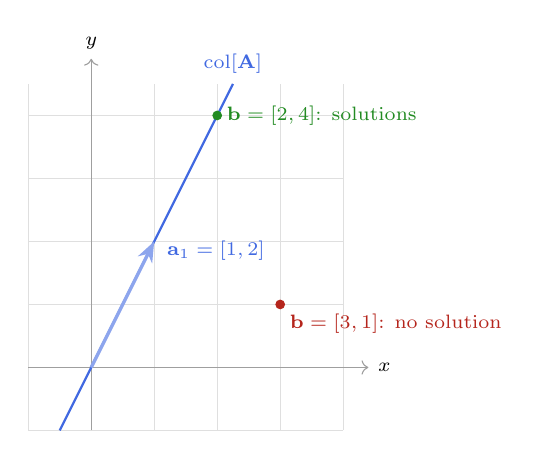
\begin{tikzpicture}[scale=0.8]
  \draw[step=1cm,gray!25,very thin] (-1,-1) grid (4,4.5);
  \draw[axisline] (-1,0) -- (4.4,0) node[right,font=\scriptsize,black]{$x$};
  \draw[axisline] (0,-1) -- (0,4.9) node[above,font=\scriptsize,black]{$y$};
  \draw[RoyalBlue,thick] (-0.5,-1) -- (2.25,4.5)
       node[above,font=\scriptsize]{$\colsp{\mt{A}}$};
  \draw[vecarr,RoyalBlue!60] (0,0) -- (1,2);
  \node[right,font=\scriptsize,RoyalBlue] at (1.05,1.85) {$\vc{a}_1=[1,2]$};
  \fill[BrickRed] (3,1) circle (2.2pt)
       node[below right,font=\scriptsize]{$\vc{b}=[3,1]$: no solution};
  \fill[ForestGreen] (2,4) circle (2.2pt)
       node[right,font=\scriptsize]{$\vc{b}=[2,4]$: solutions};
\end{tikzpicture}
\end{center}

\noindent The vector unit's review sorted the outcomes of a $2\times2$ system
into three cases: one solution, none, or infinitely many. The first half of
that sorting is now a statement about any system of any size: \emph{no
solution} means exactly that $\vc{b}$ lies outside $\colsp{\mt{A}}$. The other
half, one solution versus infinitely many, is decided by a second subspace,
which arrives in Part 6.

%------------------------------------------------------------------------------
\subsection{Examples}
%------------------------------------------------------------------------------
\begin{ex}
\label{ex:colspaces}
Five column spaces, read off the columns.
\begin{enumerate}[label=(\alph*),leftmargin=2em,itemsep=3pt]
  \item $\mt{I}=\begin{bmatrix}1&0\\0&1\end{bmatrix}$: the columns
        $\vc{e}_1,\vc{e}_2$ span $\R^{2}$, so $\colsp{\mt{I}}=\R^{2}$, and
        $\mt{I}\vc{x}=\vc{b}$ is solvable for every $\vc{b}$ (by
        $\vc{x}=\vc{b}$).
  \item $\begin{bmatrix}1&2\\2&4\end{bmatrix}$: the line through $[\,1,2\,]$,
        as in Example~\ref{ex:p5}.
  \item $\begin{bmatrix}1&0\\0&1\\0&0\end{bmatrix}\in\R^{3\times2}$: the
        columns are $\vc{e}_1,\vc{e}_2$ of $\R^{3}$, so the column space is
        the $xy$-plane, $\{[\,x,y,0\,]\}$. The system with $\vc{b}=[\,1,2,0\,]$
        is solvable; with $\vc{b}=[\,1,2,3\,]$ it is not, since nothing the
        matrix produces has a nonzero third entry.
  \item $\begin{bmatrix}1&1&2\\0&1&1\end{bmatrix}\in\R^{2\times3}$: the first
        two columns already span $\R^{2}$ (they are independent, by the test
        of the vector unit's \S18.5: $D=1\cdot1-0\cdot1=1\neq0$), so the column
        space is all of $\R^{2}$. The third column adds nothing new.
  \item The $2\times2$ zero matrix: every product is $\vc{0}$, so the column
        space is $\{\vc{0}\}$.
\end{enumerate}
\end{ex}

\begin{rmk}
Part (d) shows something worth stating once. A column that is a linear
combination of the others does not enlarge the column space: it is already in
the span of the rest. So a matrix can have many columns and a small column
space, and the number that matters is not how many columns there are but how
many \emph{independent directions} they contain. That number is the rank, in
\S12.
\end{rmk}

%==============================================================================
\section{The row space}
%==============================================================================

%------------------------------------------------------------------------------
\subsection{The definition}
%------------------------------------------------------------------------------
A matrix has rows as well as columns, and the rows span something too. Row $i$
of $\mt{A}\in\R^{m\times n}$ has one entry per column, so the rows
$\vc{r}_1,\dots,\vc{r}_m$ are vectors in $\R^{n}$.

\begin{defn}[Row space]
The \textbf{row space} of $\mt{A}\in\R^{m\times n}$ is the span of its rows:
\[
  \rowsp{\mt{A}} \;=\; \spanop\{\vc{r}_1,\dots,\vc{r}_m\} .
\]
It is a set of vectors in $\R^{n}$.
\end{defn}

\noindent Transposing turns rows into columns (\S6.3), so the rows of
$\mt{A}$ are exactly the columns of $\mt{A}\T$, and
\[
  \rowsp{\mt{A}} \;=\; \colsp{\mt{A}\T} .
\]
That one line gives everything \S10 proved, for free: the row space is a
subspace of $\R^{n}$, because it is the column space of the $n\times m$ matrix
$\mt{A}\T$.

%------------------------------------------------------------------------------
\subsection{Two different homes}
%------------------------------------------------------------------------------
For a matrix that is not square, the column space and the row space are not
even in the same space.

\begin{ex}
Let $\mt{A}=\begin{bmatrix}1&0&2\\0&1&3\end{bmatrix}\in\R^{2\times3}$. The
columns $[\,1,0\,]$, $[\,0,1\,]$, $[\,2,3\,]$ are vectors in $\R^{2}$, and the
first two already span it, so $\colsp{\mt{A}}=\R^{2}$. The rows
$[\,1,0,2\,]$ and $[\,0,1,3\,]$ are vectors in $\R^{3}$. Neither is a multiple of
the other, so they span a plane through the origin in $\R^{3}$. One subspace is
the whole of $\R^{2}$; the other is a plane inside $\R^{3}$.
\end{ex}

\begin{warn}[Column space and row space are different subspaces]
Even for a square matrix, where both live in $\R^{n}$, the two are usually
different. Take
$\mt{A}=\begin{bmatrix}1&2\\0&0\end{bmatrix}$. Its columns $[\,1,0\,]$ and
$[\,2,0\,]$ span the $x$-axis, so $\colsp{\mt{A}}$ is the $x$-axis. Its rows are
$[\,1,2\,]$ and $[\,0,0\,]$, so $\rowsp{\mt{A}}$ is the line through
$[\,1,2\,]$. Two different lines. They coincide when $\mt{A}$ is symmetric,
since then $\mt{A}\T=\mt{A}$; that is why Example~\ref{ex:p5}'s matrix, which
is symmetric, has the same line for both.
\end{warn}

%------------------------------------------------------------------------------
\subsection{What the row space does}
%------------------------------------------------------------------------------
The column space is what the column reading of $\mt{A}\vc{x}$ produces. The
row space belongs to the \emph{row} reading (\S2.3): the $i$-th entry of
$\mt{A}\vc{x}$ is the dot product of row $i$ with $\vc{x}$,
\[
  (\mt{A}\vc{x})_i \;=\; \langle\vc{r}_i,\vc{x}\rangle .
\]
So the rows are the directions along which the matrix \emph{measures} its
input. A vector orthogonal to every row gets measured as zero in every slot,
so it is sent to $\vc{0}$. Those vectors form a subspace of their own, the
null space, and \S31 shows that it is exactly the set of vectors orthogonal to
the row space.

%==============================================================================
\section{Rank}
%==============================================================================

%------------------------------------------------------------------------------
\subsection{The definition}
%------------------------------------------------------------------------------
\lookback The dimension of a subspace is the number of vectors in any basis for
it (\S17, and \S24 in $\R^{n}$). A line through the origin has dimension $1$, a
plane through the origin dimension $2$, the subspace $\{\vc{0}\}$ dimension $0$.

\begin{defn}[Rank]
The \textbf{rank} of $\mt{A}\in\R^{m\times n}$ is the dimension of its column
space:
\[
  \rank(\mt{A}) \;=\; \dim\colsp{\mt{A}} .
\]
\end{defn}

%------------------------------------------------------------------------------
\subsection{Rank counts independent columns}
%------------------------------------------------------------------------------
A basis for the column space can always be chosen from among the columns
themselves. Start with all $n$ columns. If they are dependent, one of them is a
combination of the others (the vector unit, \S18.4); delete it, and by the
remark in \S10.4 the span does not change. Repeat until what remains is
independent. What remains still spans $\colsp{\mt{A}}$ and is independent, so it
is a basis. Hence:

\begin{center}
\fcolorbox{RoyalBlue!45}{RoyalBlue!7}{%
\begin{minipage}{0.88\textwidth}
\centering
$\rank(\mt{A})$ is the largest number of linearly independent columns of
$\mt{A}$.
\end{minipage}}
\end{center}

\noindent Two bounds follow at once. There are only $n$ columns, so
$\rank(\mt{A})\le n$. And $\colsp{\mt{A}}$ is a subspace of $\R^{m}$, which
cannot hold more than $m$ independent vectors, so $\rank(\mt{A})\le m$.
Together,
\[
  \rank(\mt{A}) \;\le\; \min(m,n) .
\]

%------------------------------------------------------------------------------
\subsection{Examples, by inspection}
%------------------------------------------------------------------------------
For small matrices the rank can be read off without computation, by spotting
which columns are combinations of which.

\begin{ex}
\label{ex:ranks}
\leavevmode
\begin{enumerate}[label=(\alph*),leftmargin=2em,itemsep=3pt]
  \item Any zero matrix has rank $0$: its column space is $\{\vc{0}\}$.
  \item $\mt{I}_n$ has rank $n$: its columns $\vc{e}_1,\dots,\vc{e}_n$ are
        independent.
  \item $\begin{bmatrix}1&2\\2&4\end{bmatrix}$ has rank $1$: the second column
        is twice the first, and the first is not zero.
  \item $\begin{bmatrix}1&2\\3&4\end{bmatrix}$ has rank $2$: the columns
        $[\,1,3\,]$ and $[\,2,4\,]$ are not parallel ($D=4-6=-2\neq0$).
  \item $\begin{bmatrix}1&0&1\\0&1&1\\1&1&2\end{bmatrix}$ has rank $2$: the
        third column is the sum of the first two, and the first two are not
        parallel.
  \item The $3\times2$ matrix
        $\begin{bmatrix}1&0\\0&1\\0&0\end{bmatrix}$ has rank $2=\min(3,2)$.
  \item An outer product has rank $1$. With $\vc{u}=[\,1,2,3\,]$ and
        $\vc{v}=[\,1,-1\,]$,
        \[
          \vc{u}\vc{v}\T=
          \begin{bmatrix}1&-1\\2&-2\\3&-3\end{bmatrix},
        \]
        and in general column $j$ of $\vc{u}\vc{v}\T$ is $v_j\vc{u}$ (\S7.2).
        Every column is a multiple of $\vc{u}$, so when $\vc{u}$ and $\vc{v}$
        are nonzero the column space is the line through $\vc{u}$.
\end{enumerate}
\end{ex}

%------------------------------------------------------------------------------
\subsection{Row rank}
%------------------------------------------------------------------------------
The rows could be counted the same way: $\dim\rowsp{\mt{A}}$ is the largest
number of independent rows. Nothing in the definitions suggests that this
should equal the rank. It does.

For a $2\times2$ matrix
$\mt{A}=\begin{bmatrix}a&b\\c&d\end{bmatrix}$ it can be checked directly. The
vector unit's test (\S18.5) says the columns $[\,a,c\,]$ and $[\,b,d\,]$ are
independent exactly when
\[
  D_{\text{cols}} \;=\; a\cdot d - c\cdot b \;\neq\; 0 ,
\]
and the rows $[\,a,b\,]$ and $[\,c,d\,]$ are independent exactly when
\[
  D_{\text{rows}} \;=\; a\cdot d - b\cdot c \;\neq\; 0 .
\]
These are the same number. So the columns are independent exactly when the
rows are, and both have rank $2$ together. If they are dependent, the matrix
has rank $1$ both ways unless it is the zero matrix, which has rank $0$ both
ways.

\begin{thm}[Row rank equals column rank]
For every $\mt{A}\in\R^{m\times n}$,
$\dim\rowsp{\mt{A}} = \dim\colsp{\mt{A}} = \rank(\mt{A})$.
\end{thm}

\noindent The $2\times2$ case was just checked. The general proof needs
the null space and is given in \S33.3.

\begin{rmk}
It is a stronger statement than it looks. A $2\times100$ matrix has one hundred
columns in $\R^{2}$ and two rows in $\R^{100}$. The theorem says that however
the entries are chosen, the hundred columns span exactly as many dimensions as
the two rows do. Since there are only two rows, that is at most two, which is
also clear from the columns' side, since they live in $\R^{2}$. The theorem is
that the two counts agree \emph{exactly}, not just in their upper bound.
\end{rmk}

%==============================================================================
\section{A matrix moves the plane}
%==============================================================================
The column space is a static object: a set of vectors. This section adopts the
point of view that makes it dynamic. A matrix \emph{does} something to a
vector: it takes it in and hands back another.

%------------------------------------------------------------------------------
\subsection{A matrix as a function}
%------------------------------------------------------------------------------
Fix $\mt{A}\in\R^{m\times n}$. For each input $\vc{x}\in\R^{n}$ the product
$\mt{A}\vc{x}$ is a vector in $\R^{m}$. So $\mt{A}$ defines a function
\[
  \vc{x}\;\longmapsto\;\mt{A}\vc{x},
  \qquad
  \R^{n}\longrightarrow\R^{m},
\]
with inputs in $\R^{n}$ and outputs in $\R^{m}$. Its set of outputs is
$\colsp{\mt{A}}$. When $m=n=2$, the inputs and outputs are both points of the
plane, and we can watch the matrix pick each point up and set it down
somewhere else.

%------------------------------------------------------------------------------
\subsection{Linearity}
%------------------------------------------------------------------------------
Two of the laws in \S8.4, M2 and M4, become statements about this function once
the vectors are read as $n\times1$ matrices.

\begin{thm}
\label{thm:linear}
For every $\mt{A}\in\R^{m\times n}$, all $\vc{x},\vc{y}\in\R^{n}$ and every
scalar $c$,
\[
  \mt{A}(\vc{x}+\vc{y}) = \mt{A}\vc{x}+\mt{A}\vc{y},
  \qquad
  \mt{A}(c\vc{x}) = c\,(\mt{A}\vc{x}) .
\]
\end{thm}

\noindent These two properties have a name.

\begin{defn}[Linear transformation]
A function $T:\R^{n}\to\R^{m}$ is \textbf{linear}, or a \textbf{linear
transformation}, if
\[
  T(\vc{x}+\vc{y}) = T(\vc{x})+T(\vc{y})
  \qquad\text{and}\qquad
  T(c\vc{x}) = c\,T(\vc{x})
\]
for all $\vc{x},\vc{y}\in\R^{n}$ and all scalars $c$.
\end{defn}

\noindent So every matrix gives a linear transformation. One consequence is
immediate and will matter in Part 3: taking $c=0$ gives $T(\vc{0})=\vc{0}$.
\emph{A linear transformation never moves the origin.}

%------------------------------------------------------------------------------
\subsection{Column \texorpdfstring{$j$}{j} is where \texorpdfstring{$\vc{e}_j$}{e\_j} goes}
%------------------------------------------------------------------------------
Feed the standard basis vector $\vc{e}_j$ into $\mt{A}$. By the column
reading, $\mt{A}\vc{e}_j=0\vc{a}_1+\cdots+1\vc{a}_j+\cdots+0\vc{a}_n=\vc{a}_j$.

\begin{center}
\fcolorbox{RoyalBlue!45}{RoyalBlue!7}{%
\begin{minipage}{0.88\textwidth}
\centering
Column $j$ of $\mt{A}$ is $\mt{A}\vc{e}_j$, the place where $\mt{A}$ sends
the $j$-th standard basis vector.
\end{minipage}}
\end{center}

\noindent The converse is what makes this useful. Suppose $T:\R^{n}\to\R^{m}$
is \emph{any} linear transformation, described in words or by a formula, with
no matrix in sight. Write the input in the standard basis,
$\vc{x}=x_1\vc{e}_1+\cdots+x_n\vc{e}_n$, and apply linearity:
\[
  T(\vc{x})
  = x_1T(\vc{e}_1)+\cdots+x_nT(\vc{e}_n)
  = \begin{bmatrix}
      T(\vc{e}_1) & \cdots & T(\vc{e}_n)
    \end{bmatrix}\vc{x},
\]
the last step being the column reading again. So $T$ is multiplication by the
matrix whose columns are $T(\vc{e}_1),\dots,T(\vc{e}_n)$.

\begin{thm}
A linear transformation $T:\R^{n}\to\R^{m}$ is completely determined by the
$n$ vectors $T(\vc{e}_1),\dots,T(\vc{e}_n)$. It is multiplication by the matrix
whose $j$-th column is $T(\vc{e}_j)$.
\end{thm}

\begin{ex}
Let $T:\R^{2}\to\R^{2}$ be $T([\,x,y\,])=[\,2x,\ x+y\,]$. It is linear: each
output entry is a combination of $x$ and $y$ with fixed coefficients.
$T(\vc{e}_1)=T([\,1,0\,])=[\,2,1\,]$ and $T(\vc{e}_2)=T([\,0,1\,])=[\,0,1\,]$,
so
\[
  T \text{ is multiplication by }
  \begin{bmatrix}2&0\\1&1\end{bmatrix},
  \qquad\text{and indeed}\qquad
  \begin{bmatrix}2&0\\1&1\end{bmatrix}
  \begin{bmatrix}x\\y\end{bmatrix}
  =\begin{bmatrix}2x\\x+y\end{bmatrix}. \quad\checkmark
\]
\end{ex}

\noindent This is the recipe Part 3 runs on. To build the matrix of a
geometric motion of the plane, decide where the motion sends $\vc{e}_1$ and
$\vc{e}_2$, and write those two vectors down as columns.

\begin{rmk}
Linear transformations between spaces other than $\R^{n}$, and the reason
matrix multiplication is defined the way \S8.1 defined it, are taken up near
the end of the course. Here a matrix acting on $\R^{n}$ is all we need.
\end{rmk}

%------------------------------------------------------------------------------
\subsection{What happens to the grid}
%------------------------------------------------------------------------------
In the plane, the unit square has corners $\vc{0}$, $\vc{e}_1$, $\vc{e}_2$ and
$\vc{e}_1+\vc{e}_2$. A $2\times2$ matrix sends them to $\vc{0}$, $\vc{a}_1$,
$\vc{a}_2$ and $\vc{a}_1+\vc{a}_2$, and by linearity it sends every point
$x_1\vc{e}_1+x_2\vc{e}_2$ of the square to the point $x_1\vc{a}_1+x_2\vc{a}_2$.
So:

\begin{itemize}[leftmargin=1.4em,itemsep=3pt]
  \item the unit square goes to the parallelogram with sides $\vc{a}_1$ and
        $\vc{a}_2$;
  \item the whole coordinate grid goes to a grid of parallelograms, its lines
        running along $\vc{a}_1$ and $\vc{a}_2$, still parallel and still
        evenly spaced;
  \item the origin stays where it is, and lines through the origin go to lines
        through the origin (or, if the matrix crushes them, to the origin
        itself).
\end{itemize}

\noindent The figure shows $\mt{A}=\begin{bmatrix}2&1\\1&2\end{bmatrix}$. The
letter F drawn in the unit square is carried along with it, so that the motion
of the whole plane can be seen in one shape.

\begin{center}
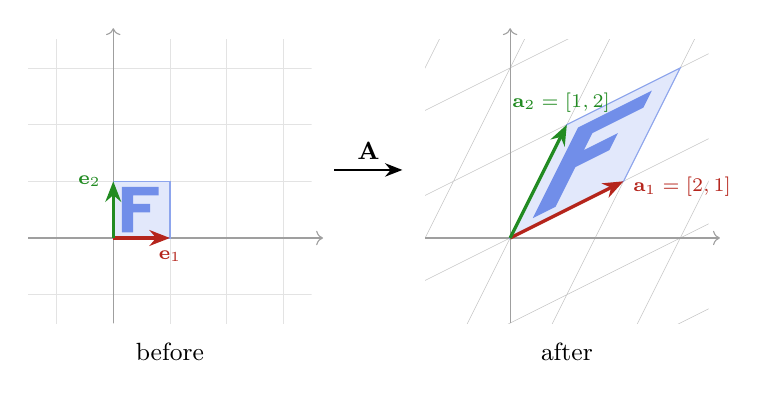
\begin{tikzpicture}[scale=0.72]
  \actionpic{1}{0}{0}{1}
  \draw[vecarr,BrickRed] (0,0) -- (1,0);
  \draw[vecarr,ForestGreen] (0,0) -- (0,1);
  \node[below,font=\scriptsize,BrickRed] at (1,-0.05) {$\vc{e}_1$};
  \node[left,font=\scriptsize,ForestGreen] at (-0.05,1) {$\vc{e}_2$};
  \node[font=\small] at (1,-2.0) {before};
  \draw[thinarr] (3.9,1.2) -- (5.1,1.2) node[midway,above,font=\small]{$\mt{A}$};
  \begin{scope}[xshift=7cm]
    \begin{scope}
      \clip (-1.5,-1.5) rectangle (3.5,3.5);
      \begin{scope}[cm={2,1,1,2,(0,0)}]
        \draw[step=1cm,gray!45,very thin] (-4,-4) grid (4,4);
      \end{scope}
    \end{scope}
    \draw[axisline] (-1.5,0) -- (3.7,0);
    \draw[axisline] (0,-1.5) -- (0,3.7);
    \begin{scope}[cm={2,1,1,2,(0,0)}]
      \fill[RoyalBlue!15] (0,0) -- (1,0) -- (1,1) -- (0,1) -- cycle;
      \draw[RoyalBlue!60] (0,0) -- (1,0) -- (1,1) -- (0,1) -- cycle;
      \fill[RoyalBlue!75] \Fshape;
    \end{scope}
    \draw[vecarr,BrickRed] (0,0) -- (2,1);
    \draw[vecarr,ForestGreen] (0,0) -- (1,2);
    \node[right,font=\scriptsize,BrickRed] at (2,0.9) {$\vc{a}_1=[2,1]$};
    \node[above,font=\scriptsize,ForestGreen] at (0.9,2.05) {$\vc{a}_2=[1,2]$};
    \node[font=\small] at (1,-2.0) {after};
  \end{scope}
\end{tikzpicture}
\end{center}

%==============================================================================
\section{The \texorpdfstring{$2\times2$}{2x2} determinant}
%==============================================================================

%------------------------------------------------------------------------------
\subsection{The number \texorpdfstring{$D$}{D}, named}
%------------------------------------------------------------------------------
\lookback The vector unit's \S18.5 found a single number that decides whether
two vectors $\vc{u},\vc{v}\in\R^{2}$ span the plane:
$D=u_1v_2-u_2v_1$, nonzero exactly when they do. It closed with the promise that
such a number ``is worth having a name, and it has one.'' Here is the name.
Put $\vc{u}$ and $\vc{v}$ in as the columns of a matrix.

\begin{defn}[Determinant of a $2\times2$ matrix]
The \textbf{determinant} of $\mt{A}=\begin{bmatrix}a&b\\c&d\end{bmatrix}$ is
the number
\[
  \det(\mt{A}) \;=\; ad-bc .
\]
\end{defn}

\noindent ``Down the main diagonal, minus up the other diagonal.'' With columns
$[\,a,c\,]$ and $[\,b,d\,]$ this is exactly the vector unit's $D$.

\begin{ex}
\label{ex:dets}
\[
  \det\begin{bmatrix}2&1\\1&2\end{bmatrix}=4-1=3,\qquad
  \det\begin{bmatrix}1&2\\2&4\end{bmatrix}=4-4=0,\qquad
  \det\begin{bmatrix}0&1\\1&0\end{bmatrix}=0-1=-1,\qquad
  \det\mt{I}=1 .
\]
\end{ex}

%------------------------------------------------------------------------------
\subsection{The determinant decides the rank}
%------------------------------------------------------------------------------
Everything \S10--\S12 established for a $2\times2$ matrix now collapses into one
test.

\begin{thm}
\label{thm:det-rank}
For $\mt{A}\in\R^{2\times2}$ the following are equivalent:
\begin{enumerate}[label=(\roman*),leftmargin=2.2em,itemsep=2pt]
  \item $\det(\mt{A})\neq0$;
  \item the columns of $\mt{A}$ are linearly independent;
  \item $\rank(\mt{A})=2$;
  \item $\colsp{\mt{A}}=\R^{2}$;
  \item $\mt{A}\vc{x}=\vc{b}$ has a solution for every $\vc{b}\in\R^{2}$.
\end{enumerate}
\end{thm}

\begin{proof}
(i)$\iff$(ii) is the vector unit's \S18.5. (ii)$\iff$(iii) by \S12.2. (ii)
gives (iv) because two independent vectors span $\R^{2}$ (\S18.5 again), and
(iv) gives (iii) since $\dim\R^{2}=2$. (iv)$\iff$(v) is the solvability
theorem of \S10.3.
\end{proof}

\noindent When $\det(\mt{A})=0$ the rank is $1$ or $0$, and it is $0$ only for
the zero matrix. One table holds the whole picture.

\begin{center}
\renewcommand{\arraystretch}{1.35}
\begin{tabular}{@{}c c l l@{}}
\toprule
$\rank(\mt{A})$ & $\det(\mt{A})$ & $\colsp{\mt{A}}$ & what $\mt{A}$ does to the plane \\
\midrule
$2$ & $\neq0$ & $\R^{2}$ & moves it onto all of itself \\
$1$ & $0$ & a line through $\vc{0}$ & flattens it onto that line \\
$0$ & $0$ & $\{\vc{0}\}$ & crushes it to the origin \\
\bottomrule
\end{tabular}
\end{center}

%------------------------------------------------------------------------------
\subsection{The size of the determinant: area}
%------------------------------------------------------------------------------
In \S13.4 the unit square, of area $1$, became the parallelogram with sides
$\vc{a}_1$ and $\vc{a}_2$. The determinant measures that parallelogram:
\[
  \text{area of the parallelogram with sides } \vc{a}_1,\vc{a}_2
  \;=\; |\det(\mt{A})| .
\]
This is stated here and derived in \S23 from base times height. For
$\mt{A}=\begin{bmatrix}2&1\\1&2\end{bmatrix}$ of \S13.4, the parallelogram with
corners $\vc{0}$, $[\,2,1\,]$, $[\,3,3\,]$, $[\,1,2\,]$ has area $3$, and
$\det(\mt{A})=3$.

And it is not only the unit square. Every square of the grid is carried to a
copy of the same parallelogram, so every region of the plane has its area
multiplied by the same factor $|\det(\mt{A})|$. The determinant is the
\emph{area scale factor} of the matrix.

%------------------------------------------------------------------------------
\subsection{The sign of the determinant: orientation}
%------------------------------------------------------------------------------
The area is $|\det(\mt{A})|$; the sign carries separate information. Turning
from $\vc{e}_1$ to $\vc{e}_2$ is a quarter-turn counterclockwise.
\begin{itemize}[leftmargin=1.4em,itemsep=3pt]
  \item If $\det(\mt{A})>0$, turning from $\vc{a}_1$ to $\vc{a}_2$ (the short
        way) is also counterclockwise. The plane is moved without being turned
        over.
  \item If $\det(\mt{A})<0$, turning from $\vc{a}_1$ to $\vc{a}_2$ is
        clockwise. The plane has been flipped, as in a mirror, and the letter F
        comes out reversed.
\end{itemize}

\begin{center}
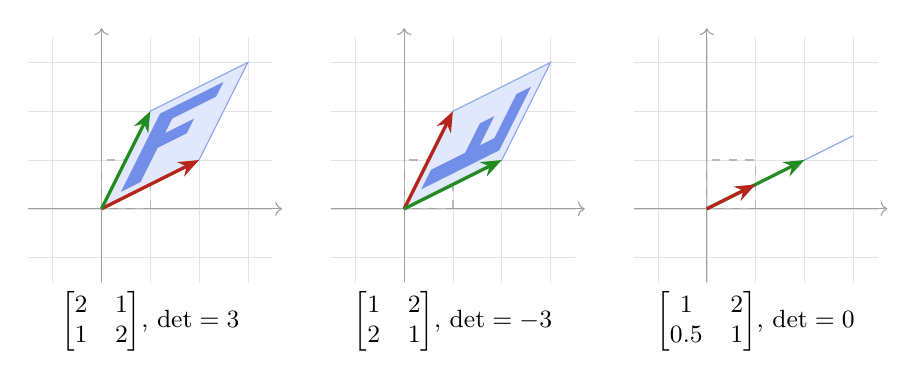
\begin{tikzpicture}[scale=0.62]
  \actionpic{2}{1}{1}{2}
  \draw[vecarr,BrickRed] (0,0) -- (2,1);
  \draw[vecarr,ForestGreen] (0,0) -- (1,2);
  \node[font=\small,align=center] at (1,-2.3)
       {$\begin{bmatrix}2&1\\1&2\end{bmatrix}$, $\det=3$};
  \begin{scope}[xshift=6.2cm]
    \actionpic{1}{2}{2}{1}
    \draw[vecarr,BrickRed] (0,0) -- (1,2);
    \draw[vecarr,ForestGreen] (0,0) -- (2,1);
    \node[font=\small,align=center] at (1,-2.3)
         {$\begin{bmatrix}1&2\\2&1\end{bmatrix}$, $\det=-3$};
  \end{scope}
  \begin{scope}[xshift=12.4cm]
    \actionpic{1}{2}{0.5}{1}
    \draw[vecarr,ForestGreen] (0,0) -- (2,1);
    \draw[vecarr,BrickRed] (0,0) -- (1,0.5);
    \node[font=\small,align=center] at (1,-2.3)
         {$\begin{bmatrix}1&2\\0.5&1\end{bmatrix}$, $\det=0$};
  \end{scope}
\end{tikzpicture}
\end{center}

\noindent In each picture the red arrow is $\mt{A}\vc{e}_1$ and the green arrow
is $\mt{A}\vc{e}_2$. On the left, area $3$ and the F reads correctly. In the
middle, the columns of the left matrix have been swapped: the same parallelogram,
area $3$ again, but the F is mirrored and the determinant is $-3$. On the right
the columns are parallel and the square is flattened into a segment.

%------------------------------------------------------------------------------
\subsection{When the determinant is zero}
%------------------------------------------------------------------------------
A zero determinant means the parallelogram has no area: its sides are parallel,
and the plane is flattened onto the line $\colsp{\mt{A}}$. Something is lost
in the flattening, and it can be located exactly.

\begin{ex}
Take $\mt{A}=\begin{bmatrix}1&2\\2&4\end{bmatrix}$ again, with
$\det(\mt{A})=0$ and column space the line through $[\,1,2\,]$. Look at the
vector $[\,2,-1\,]$:
\[
  \begin{bmatrix}1&2\\2&4\end{bmatrix}
  \begin{bmatrix}2\\-1\end{bmatrix}
  =\begin{bmatrix}2-2\\4-4\end{bmatrix}
  =\begin{bmatrix}0\\0\end{bmatrix}.
\]
By linearity every multiple $t[\,2,-1\,]$ is sent to $\vc{0}$ too. A whole line
of the plane is crushed to a single point. And because of that, different
inputs can give the same output: $\mt{A}\vc{x}=\mt{A}\vc{y}$ whenever
$\vc{x}-\vc{y}$ lies on that line. Once the matrix has acted, there is no way
to tell those inputs apart.
\end{ex}

\noindent That line, the set of vectors a matrix sends to $\vc{0}$, is the
\emph{null space}. It is the subject of Part 6, where it settles the second
half of the question \S10.3 left open: when a system has solutions, whether it
has one or infinitely many.

%------------------------------------------------------------------------------
\subsection{Practice}
%------------------------------------------------------------------------------
\begin{enumerate}[label=\textbf{P\arabic*.},leftmargin=2.6em,itemsep=5pt]
  \item Describe $\colsp{\mt{A}}$ and $\rowsp{\mt{A}}$ for
        $\mt{A}=\begin{bmatrix}1&-1&2\\-2&2&-4\end{bmatrix}$, and give
        $\rank(\mt{A})$.
  \item For which $\vc{b}$ does
        $\begin{bmatrix}1&3\\2&6\end{bmatrix}\vc{x}=\vc{b}$ have a solution?
        Is $\vc{b}=[\,4,8\,]$ one of them? Is $\vc{b}=[\,4,7\,]$?
  \item A linear transformation $T:\R^{2}\to\R^{3}$ has
        $T(\vc{e}_1)=[\,1,0,2\,]$ and $T(\vc{e}_2)=[\,-1,3,0\,]$. Write its
        matrix and compute $T([\,2,1\,])$.
  \item Compute the determinant of
        $\begin{bmatrix}3&1\\4&2\end{bmatrix}$,
        $\begin{bmatrix}-1&0\\0&2\end{bmatrix}$ and
        $\begin{bmatrix}6&-2\\-9&3\end{bmatrix}$. For each, give the rank and
        the area of the image of the unit square, and say whether the plane is
        flipped.
  \item Find a nonzero vector that
        $\begin{bmatrix}6&-2\\-9&3\end{bmatrix}$ sends to $\vc{0}$.
\end{enumerate}

\subsubsection*{Answers}

\noindent\textbf{P1.} The columns $[\,1,-2\,]$, $[\,-1,2\,]$, $[\,2,-4\,]$
are all multiples of $[\,1,-2\,]$, so $\colsp{\mt{A}}$ is the line through
$[\,1,-2\,]$ in $\R^{2}$ and $\rank(\mt{A})=1$. The second row is $-2$ times
the first, so $\rowsp{\mt{A}}$ is the line through $[\,1,-1,2\,]$ in $\R^{3}$,
of dimension $1$, as \S12.4 requires.

\smallskip
\noindent\textbf{P2.} The column space is the line through $[\,1,2\,]$ (the
second column is $3$ times the first), i.e.\ the vectors $[\,b_1,b_2\,]$ with
$b_2=2b_1$. So $[\,4,8\,]$ is one of them (solutions exist, e.g.\
$\vc{x}=[\,4,0\,]$) and $[\,4,7\,]$ is not.

\smallskip
\noindent\textbf{P3.} The columns are the images of $\vc{e}_1$ and $\vc{e}_2$:
$\begin{bmatrix}1&-1\\0&3\\2&0\end{bmatrix}$, and
$T([\,2,1\,])=2[\,1,0,2\,]+1[\,-1,3,0\,]=[\,1,3,4\,]$.

\smallskip
\noindent\textbf{P4.} $\det=6-4=2$: rank $2$, area $2$, not flipped.
$\det=-2$: rank $2$, area $2$, flipped (the $x$-direction is reversed).
$\det=18-18=0$: the second column is $-\tfrac13$ times the first; rank $1$,
area $0$; the square is flattened, so the question of flipping does not arise.

\smallskip
\noindent\textbf{P5.} The rows are both multiples of $[\,3,-1\,]$
($6x-2y=0$ and $-9x+3y=0$ are the same equation $y=3x$), so $[\,1,3\,]$ works:
$6-6=0$ and $-9+9=0$.

\lookahead Part 3 uses \S13.3 as a construction kit. It takes the motions of
the plane one meets in geometry --- scalings, shears, rotations, reflections,
projections, and one motion that turns out not to be linear at all --- and
builds each one's matrix from where it sends $\vc{e}_1$ and $\vc{e}_2$. Then it
asks which matrices move the plane without changing any length, and finds that
the answer is a single matrix equation.

\end{document}
